%% IMPORTANT: Once working, run latex 3 times to get listoffigures to work

%% Be sure to check spelling!

%% Put **your** name and the proper due date in place

%% Copy the lstlisting and figure code as many times as you need
%% Be sure to put in your own file names if appropriate

%% Note that the \epsfig command is currently commented out - until the
%%%% files exist, processing this code without them will result in an error
%%%% so leave the comments until you have created the graphics files!

\documentclass{article}
\usepackage{amsmath}    % loads AMS-Math package
\usepackage{epsfig}     % allows PostScript files
\usepackage{listings}   % allows lstlisting environment
\usepackage{moreverb}   % allows listinginput environment
\usepackage[letterpaper, margin=0.75in]{geometry}  % set paper size/margins
\usepackage{textcomp}   % adds \interrobang, among others!

\begin{document}
\begin{center}
\rule{6.5in}{0.5mm}\\~\\
\textbf{\large EGR 103L -- Fall 2017}\\~\\
\textbf{\huge Laboratory 8 - Linear Algebra}\\~\\
Ian Hanus (ih52)\\
Lab Section 1B, Tuesday 8:30-11:20\\
5 November 2017\\~\\
{\small I understand and have adhered to all the tenets of the Duke
  Community Standard in completing every part of this assignment.  I
  understand that a violation of any part of the Standard on any part
  of this assignment can result in failure of this assignment, failure
  of this course, and/or suspension from Duke University.} 
\rule{6.5in}{0.5mm}\\
\end{center}
\tableofcontents
\listoffigures
\pagebreak
\section{Palm Problem 8.1}
\renewcommand{\arraystretch}{1.5}
\begin{center}
\begin{tabular}{|c||c|c|c|}\hline
Part & x & y & z \\ \hline \hline
$a$ & 2.4762e+00 & 4.7619e-02  & N/A\\ \hline
$b$ & -1.1818e+00  & 1.0909e+00  & N/A \\ \hline
$c$ & 3.4329e+00 & -6.0390e+00  & 4.4935e+00 \\ \hline
$d$ & 2.0035e+00 & -2.6848e+00 & 5.2312e+00 \\ \hline
\end{tabular}
\end{center}

\section{Based on Chapra Problem 8.3}
% Equations in matrix form
Equations in matrix form:
\begin{align*}
\begin{bmatrix}
0 & -7 & 5\\
0 & 4 & 7\\
-4 & 3 & -7
\end{bmatrix}
\begin{Bmatrix}
x_1\\
x_2\\
x_3
\end{Bmatrix} & =
\begin{Bmatrix}
50\\
-30\\
40
\end{Bmatrix}
\end{align*}
% Solutions for this system (x = vector)
Solutions for this system:
\begin{align*}
\begin{Bmatrix}
x_1\\
x_2\\
x_3
\end{Bmatrix} & = 
\begin{Bmatrix}
-1.5181e+01\\
-7.2464e+00\\
-1.4493e-01
\end{Bmatrix}
\end{align*}
% Transpose and inverse
Transpose of A:
\begin{align*}
\begin{bmatrix}
0 & 0 & -4\\
-7 & 4 & 3\\
5 & 7 & -7
\end{bmatrix}
\end{align*}
Inverse of A:
\begin{align*}
\begin{bmatrix}
-1.7754e-01 & -1.2319e-01 & -2.5000e-01\\
-1.0145e-01 & 7.2464e-02 & 0\\
5.7971e-02 & 1.0145e-01 & 0
\end{bmatrix}
\end{align*}
% Condition numbers
Condition numbers:
\begin{center}
1-norm condition = $6.4022e+00$\\
2-norm condition = $4.0569e+00$\\
Frobenius condition = $5.4293e+00$\\
$\infty$-condition = $7.7101e+00$\\
\end{center}
% Meaning of condition numbers
The condition numbers signify how inaccurate the solution can be. Because the condition for each fo the norms is greater than one, the system is ill-conditioned. This suggests that the solutions of the system could exhibit rounding errors. Because the magnitude of each of the condition numbers is below ten, the last digit of the solutions could exhibit roundoff errors as the logarithm of the condition numbers is between 0 and 1.
\pagebreak 

\section{Based on Chapra Problem 8.10}
% Equations in matrix form
\renewcommand*{\arraystretch}{0.5}
\begin{align*}
\begin{bmatrix}
-8.6603e-01 & 0 & 5.0000e-01 & 0 & 0 & 0\\
-5.0000e-01 & 0 & -8.6603e-01 & 0 & 0 & 0\\
8.6603e-01 & 1.0000e+00 & 0 & 1.0000e+00 & 0 & 0\\
5.0000e-01 & 0 & 0 & 0 & 1.0000e+00 & 0\\
0 & -1.0000e+00 & -5.0000e-01 & 0 & 0 & 0\\
0 & 0 & 8.6603e-01 & 0 & 0 & 1.0000e+00
\end{bmatrix}
\begin{Bmatrix}
F_1\\F_2\\F_3\\H_2\\V_2\\V_3
\end{Bmatrix}&=
\begin{Bmatrix}
0\\1000\\0\\0\\0\\0
\end{Bmatrix}
\end{align*}

% Sentence introducing the following results: 
\listinginput[1]{1}{TrussData.txt}

\section{Palm 8.5(b)}
% Discussion of whether there is a c value with easily predicted solutions
There is a c value with easily predicted solutions. For a c value of 0, x,y, and z are expected to be zero. This seems appears to be true on the graph.
% Discussion of why there are 201 points
There are 201 points instead of 200 because using 200 creates an even spacing of 0.1 between all points. This would include the c value zero. Using 201 points, the spacing is different and does not include a calculated c value of zero.

\section{Based on Palm 8.9}
% Equations in matrix form
\renewcommand*{\arraystretch}{1}
\begin{align*}
\begin{bmatrix}
-1 & 1/3 & 1/3 & 0\\
1/2 & -1 & 0 & 1/2\\
1/3 & 0 & -1 & 1/3\\
0 & 1/2 & 1/2 & -1
\end{bmatrix}
\begin{Bmatrix}
T_1\\T_2\\T_3\\T_4
\end{Bmatrix} & =
\begin{Bmatrix}
-50\\0\\-20/3\\0
\end{Bmatrix}
\end{align*}
% Sentence introducing the following results: 
The following are the temperatures at each square.
\listinginput[1]{1}{TempData.txt}

\section{Based on Palm 8.16(a)}
\begin{align*}
\begin{bmatrix}
x_1^2 & x_1 & 1\\
x_2^2 & x_2 & 1\\
x_3^2 & x_3 & 1
\end{bmatrix}
\begin{Bmatrix}
a\\b\\c
\end{Bmatrix} & =
\begin{Bmatrix}
y_1\\y_2\\y_3
\end{Bmatrix}
\end{align*}
% Sentence introducing the table of results
The following are the coefficients of the quadratics containing the given points.
\begin{center}
\[
\begin{tabular}{|c|c|c|c|}
\hline \mbox{Points} & a & b & c\\
\hline (1,4), (4,73), (5,120) & 6.00e+00 & -7.00e+00 & 5.00e+00\\
(1,4), (4,-73), (5,120) & 5.47e+01 & -2.99e+02 & 2.48e+02\\
(1,4), (4,73), (4,120) & N/A & N/A & N/A\\
(1,4), (4,73), (5,-120) & -5.40e+01 & 2.93e+02 & -2.35e+02\\ \hline
\end{tabular}
\]
\end{center}
% Table of results.

\pagebreak
\appendix
\section{Codes and Output}
% Put the name of your file in the subsection name 
% and the listinginput input
% Be sure to include the community standard in codes!
% Add \pagebreaks if they make sense
% Make as many copies as you need

\subsection{Chapra83.m}
\listinginput[1]{1}{Chapra83.m}

\subsection{Chapra810.m}
\listinginput[1]{1}{Chapra810.m}

\subsection{Palm85}
\listinginput[1]{1}{Palm85.m}

\subsection{Palm89}
\listinginput[1]{1}{Palm89.m}

\subsection{Palm816}
\listinginput[1]{1}{Palm816.m}

\pagebreak
\section{Figures}

\begin{figure}[htb!]
\begin{center}
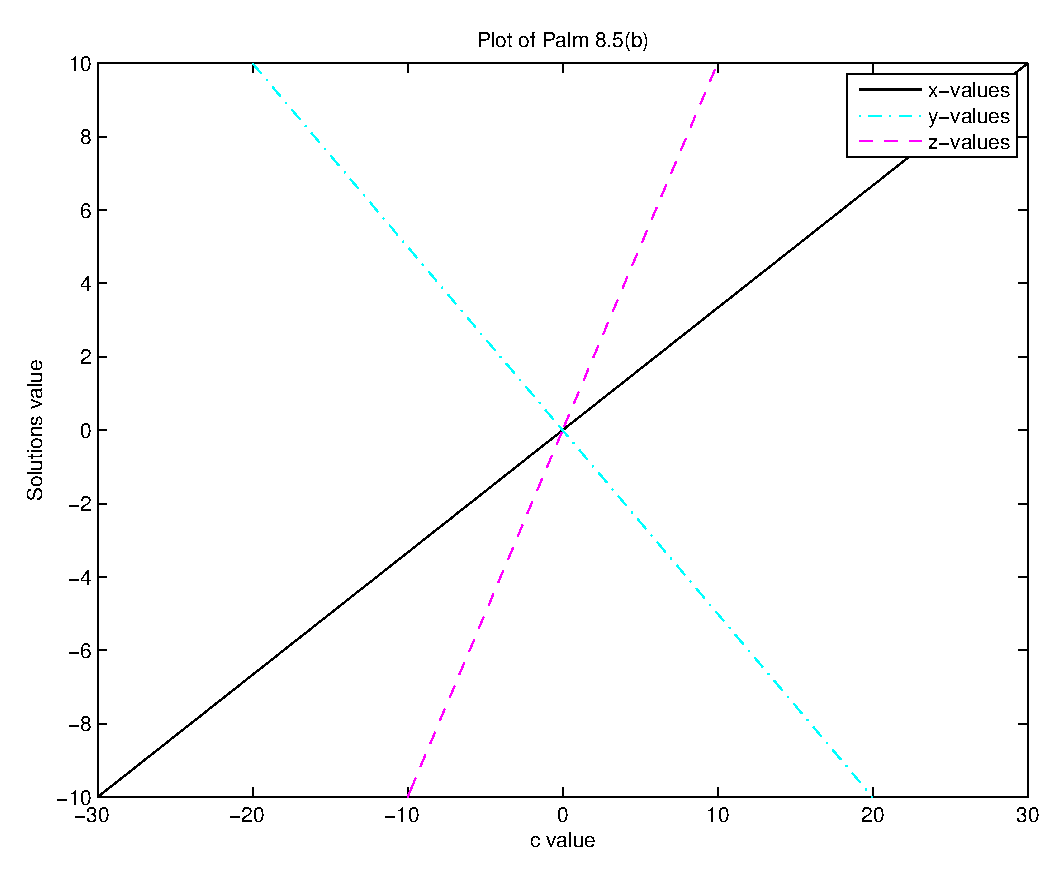
\epsfig{file=Palm85bPlot.eps, width=3.in}
\caption{Plot of Palm 8.5(b)}
\end{center}
\end{figure}

\begin{figure}[htb!]
\begin{center}
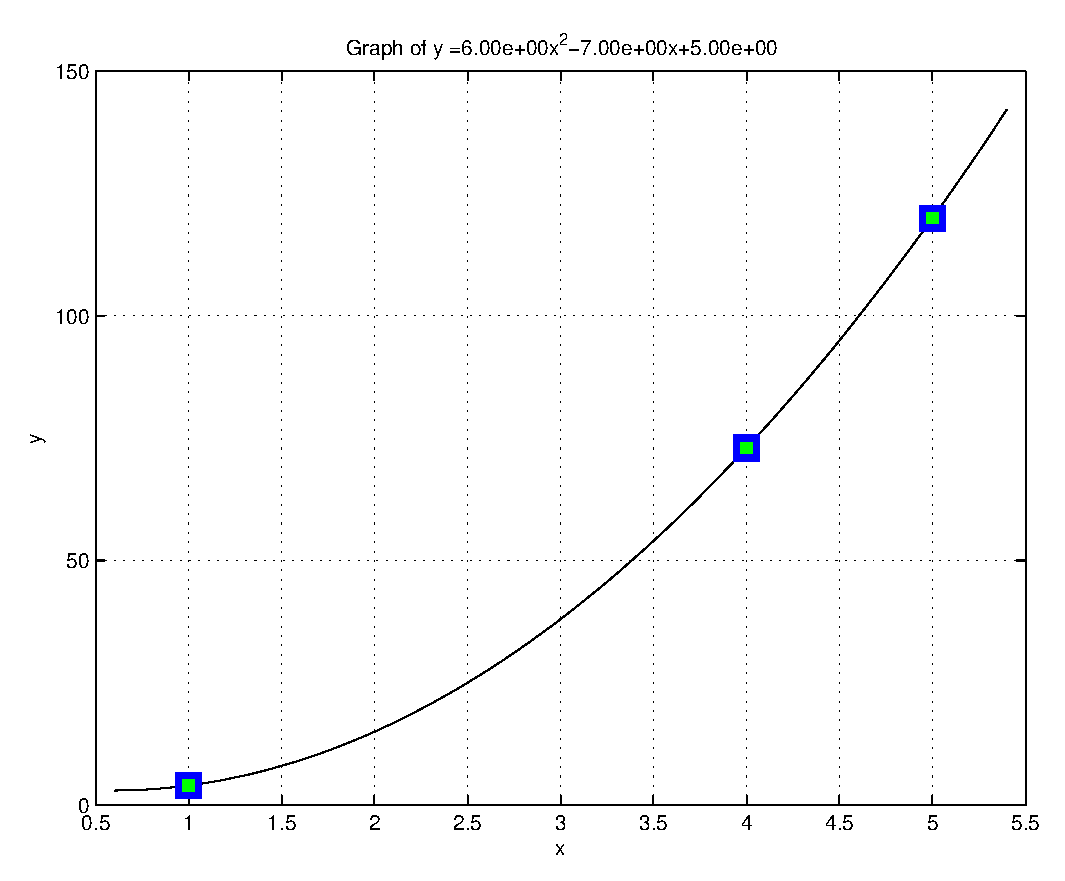
\epsfig{file=Palm816fig1.eps, width=3.in}
\caption{Plot of Polynomial for Points (1,4), (4,73), (5,120)}
\end{center}
\end{figure}

\begin{figure}[htb!]
\begin{center}
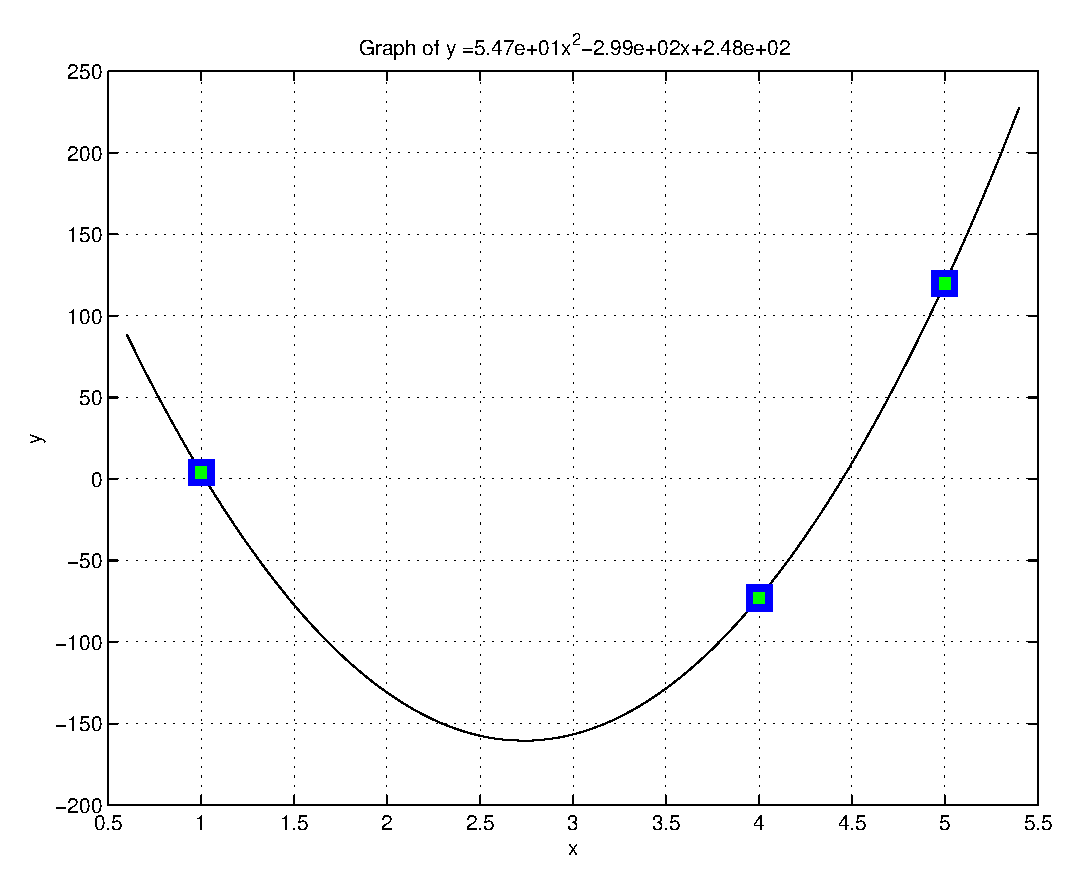
\epsfig{file=Palm816fig2.eps, width=3.in}
\caption{Plot of Polynomial for Points (1,4), (4,-73), (5,120)}
\end{center}
\end{figure}

\begin{figure}[htb!]
\begin{center}
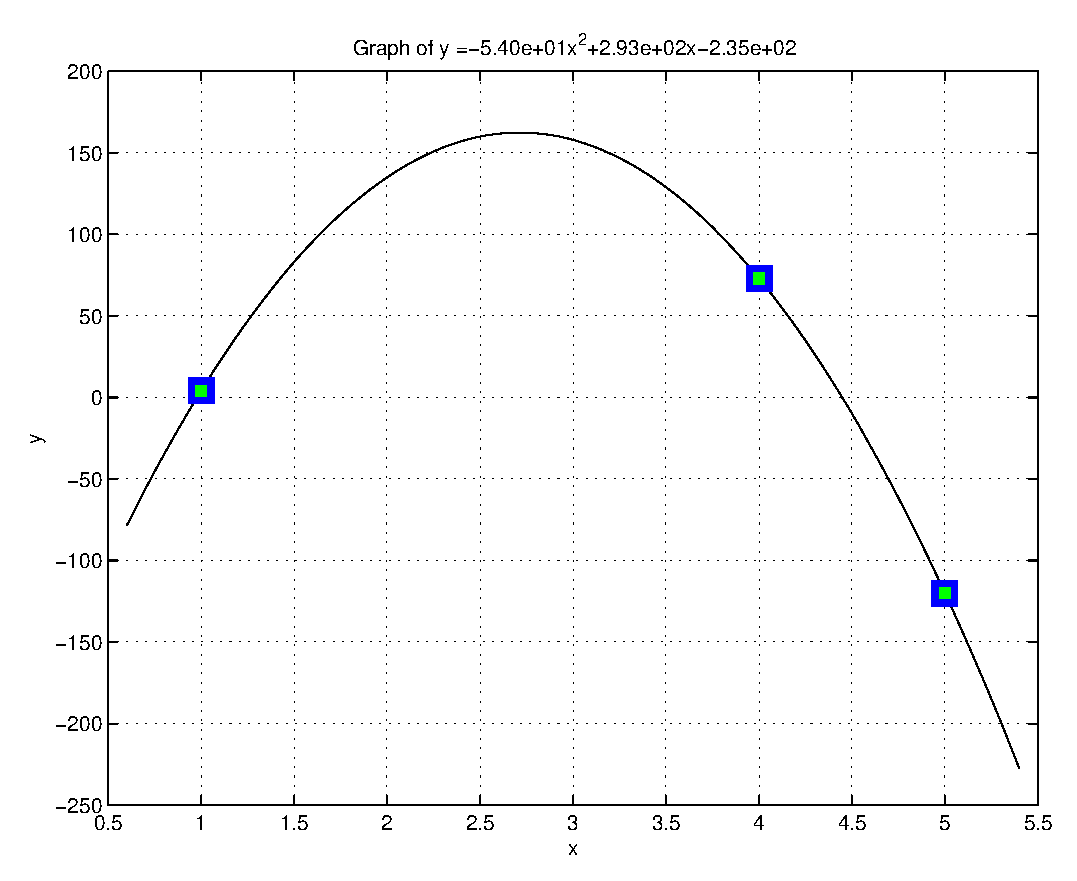
\epsfig{file=Palm816fig3.eps, width=3.in}
\caption{Plot of Polynomial for Points (1,4), (4,73), (5,-120)}
\end{center}
\end{figure}

\end{document}


